
\chapter{Solving the wave equation with the FEM} \label{fem_waveq} 
\begin{flushright} {\tiny {\color{gray} chapter\_fem3.tex}} \end{flushright}


%==============================================================================
\section{The wave equation}

[what follows is greatly inspired by \url{https://en.wikipedia.org/wiki/Wave_equation} ]

The wave equation is a second-order linear partial differential equation 
for the description of waves or standing wave fields such as mechanical waves 
(e.g. water waves, sound waves and seismic waves) or electromagnetic waves 
(including light waves). It arises in fields like acoustics, electromagnetism, and fluid dynamics. 

The wave equation is a hyperbolic partial differential equation,
and we will here focus on the scalar wave equation that 
represent the wave by a scalar $u(x,y,z,t)$.

The scalar wave equation is given by
\begin{equation}
\frac{\partial^2 u}{\partial t^2} = c^2 \left(
\frac{\partial^2 u}{\partial x^2} + 
\frac{\partial^2 u}{\partial y^2} + 
\frac{\partial^2 u}{\partial z^2} 
\right)
\end{equation}
where $c$ is a fixed non-negative real coefficient (the wave speed),
u is a scalar field representing a displacement from rest situation, e.g.
it could be gas pressure above or below normal, or the height of water in 
a pond above or below rest.

The equation states that at any given instance, at any given point, 
the acceleration of the displacement is proportional to the way the displacement's 
changes are squashed up in the surrounding area. In other words, a more pointy 
displacement gets pushed back more forcefully. 

This equation can also be written 
\begin{equation}
\frac{1}{c^2} \frac{\partial^2 u}{\partial t^2} = \Delta u
\end{equation}
or even 
\[
\Box u = 0 \qquad \text{with} \qquad \Box= \frac{1}{c^2} \frac{\partial^2 u}{\partial t^2} - \Delta
\]
in its most compact form, where $\Box$ is the d'Alembert 
operator\footnote{\url{https://en.wikipedia.org/wiki/D'Alembert_operator}}.


Solving the wave equation can be quite complicated. Still, it can be analyzed 
as a linear combination of simple solutions that are sinusoidal plane waves 
with various directions of propagation and wavelengths but all with the same propagation 
speed $c$. This analysis is possible because the wave equation is linear and homogeneous, 
so that any multiple of a solution is also a solution, and the sum of any two solutions 
is again a solution. This property is called the superposition principle in physics.


The wave equation alone does not specify a physical solution; 
a {\it unique} solution is usually obtained by setting a problem with further 
conditions, such as initial conditions, which prescribe the amplitude and phase of the wave. 
Another important class of problems occurs in enclosed spaces specified by boundary 
conditions, for which the solutions represent standing waves, or harmonics, analogous 
to the harmonics of musical instruments. 



%==============================================================================
\section{Solving the one-dimensional wave equation}

The derivation of the one-dimensional wave equation is presented 
there\footnote{\url{https://en.wikipedia.org/wiki/Wave_equation}} 
and in virtuallly every physics textbook.

It simply writes
\[
\frac{\partial^2 u}{\partial t^2} = c^2 
\frac{\partial^2 u}{\partial x^2} 
\]
or also sometimes
\[
u_{tt} = c^2 u_{xx}
\]
The one-dimensional wave equation is unusual for a partial differential equation 
in that a relatively simple general solution may be found:
\[
u(x,t)=F(x-ct)+G(x+ct)
\]
iSolutions of the 1D wave equation are sums of a right-traveling function 
$F$ and a left-traveling function $G$. 
``Traveling'' means that the shape of these individual arbitrary 
functions with respect to $x$ stays constant, however, the functions are 
translated left and right with time at the speed $c$. 
This was derived by Jean le Rond d'Alembert.

This equation is to be solved on the domain $x \in [0,L_x]$.

%-------------------------------------------
\subsection{Initial and boundary conditions}

Simply put, we need to specify the state of the system $u$ at the beginning, 
and since the domain in which the wave propagates is likely to be finite, 
also the boundary conditions.

For simplicity we will set
\begin{align}
u(x=0,t) & = 0 & \forall t\in \R^+ \\
u(x=L_x,t) & = 0 & \forall t\in \R^+ \\
u(x,0) &= u_0(x) & \forall x\in[0,L_x]\\
u_t(x,0) &= u_1(x) & \forall x\in[0,L_x]
\end{align}

%-------------------------------------------
\subsection{A simple example: a standing wave \label{ss:sw1d}}

Let us set $L_x=1$ and $c=1$. Then one of the solutions is 
given by 
\[
x(x,t)=\cos(2\pi t) \sin(2\pi x)
\]
which is periodic in time with period 1 and is called a standing wave.
We also have
\[
u_t(x,t)=-2 \pi \sin (2\pi t) \sin(2\pi x)
\]
so that 
\begin{eqnarray}
u_0(x) &=& \sin(2\pi x) \\
u_1(x) &=& 0 
\end{eqnarray}
and the boundary conditions are respected: $u(0,t)=u(1,t)=0 \quad \forall t$.

\begin{center}
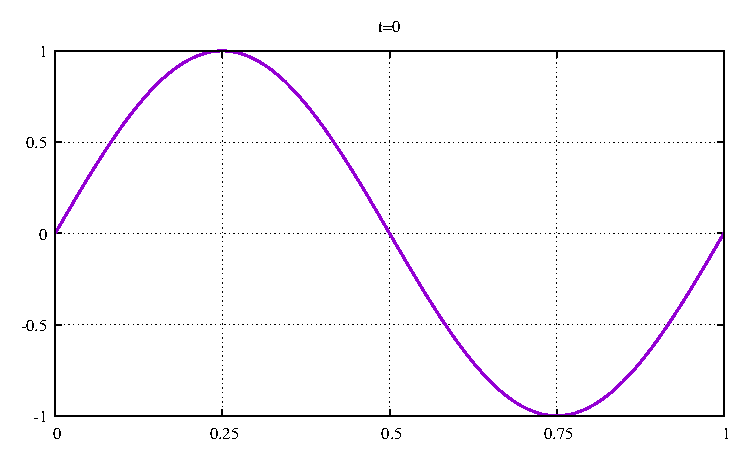
\includegraphics[width=4cm]{images/waveq/example1/u_0.pdf}
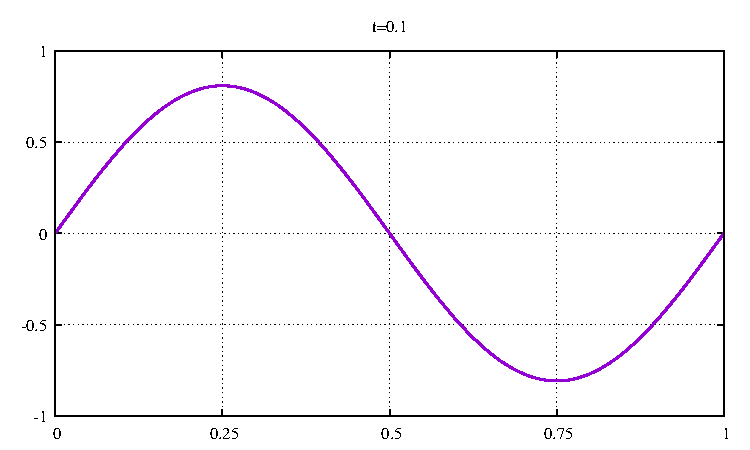
\includegraphics[width=4cm]{images/waveq/example1/u_1.pdf}
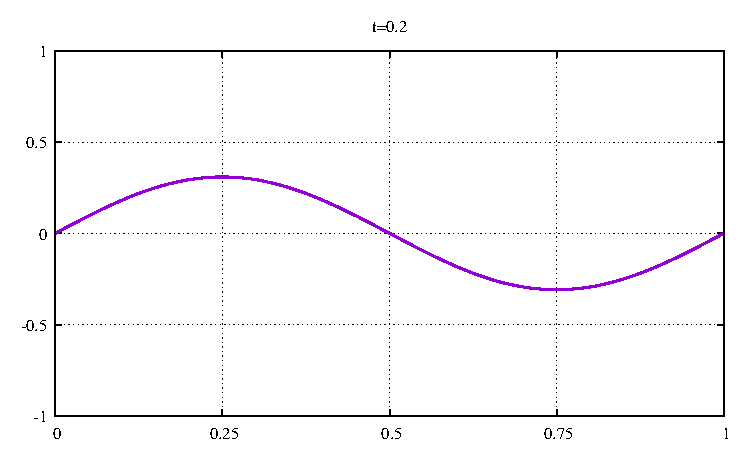
\includegraphics[width=4cm]{images/waveq/example1/u_2.pdf}
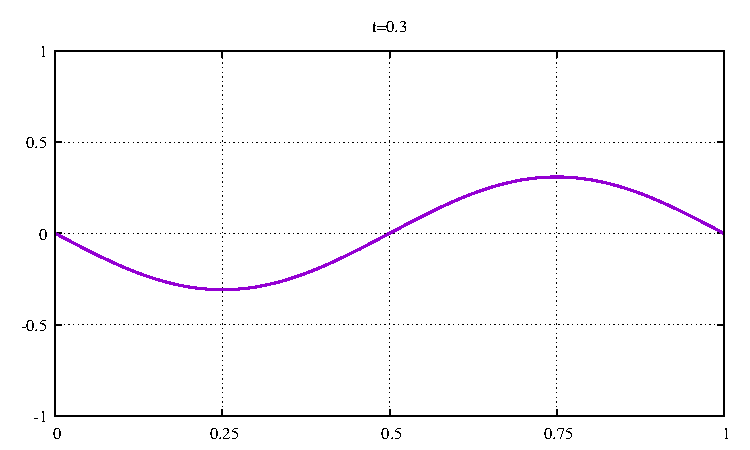
\includegraphics[width=4cm]{images/waveq/example1/u_3.pdf}\\
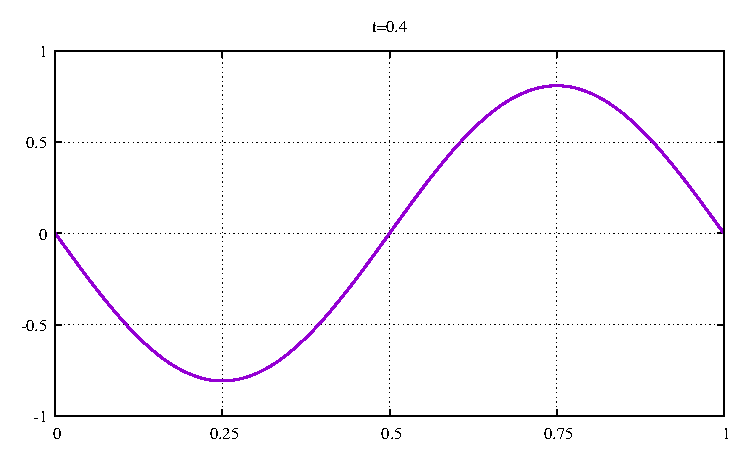
\includegraphics[width=4cm]{images/waveq/example1/u_4.pdf}
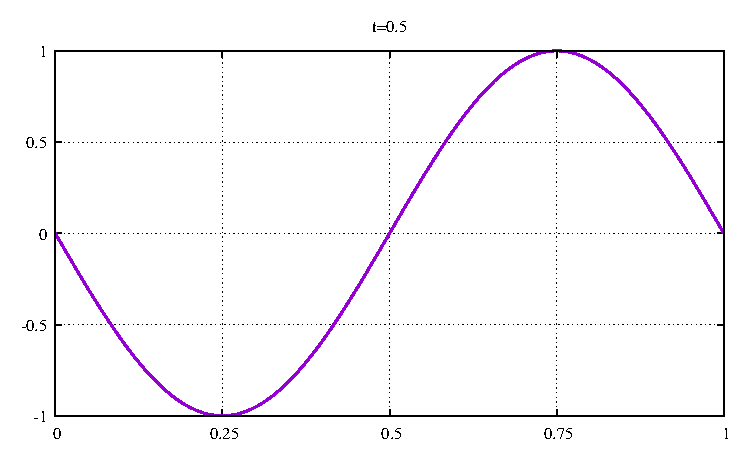
\includegraphics[width=4cm]{images/waveq/example1/u_5.pdf}
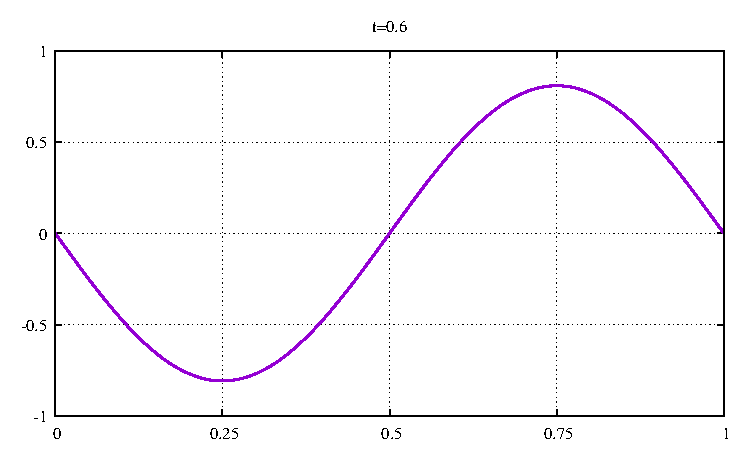
\includegraphics[width=4cm]{images/waveq/example1/u_6.pdf}
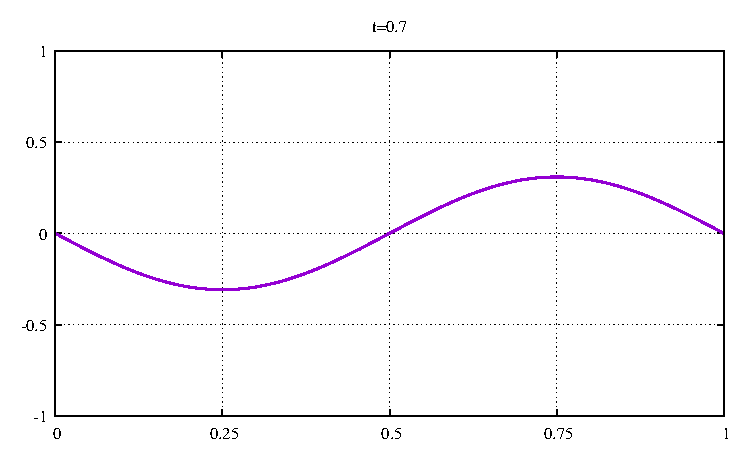
\includegraphics[width=4cm]{images/waveq/example1/u_7.pdf}\\
{\captionfont Solution at different times.}
\end{center}


{\color{red} ... include here weak form derivation and discretisation ... }


We arrive at
\begin{equation}
\M \cdot \vec{\ddot{{\cal U}}}(t) + c^2 \K \cdot \vec{\cal U}(t) = \vec{0}
\label{ss:waveq1}
\end{equation}

We can use a second-order approximation for the second-order derivative:
\[
\vec{\ddot{{\cal U}}}(t) \simeq  \frac{ \vec{\cal U}(t+dt) -2 \vec{\cal U}(t) + \vec{\cal U}(t-dt)}{dt^2}
\]
which we can substitute in Eq.~\eqref{ss:waveq1}:
\[
\M \cdot \frac{ \vec{\cal U}(t+dt) -2 \vec{\cal U}(t) + \vec{\cal U}(t-dt)}{dt^2} 
+c^2 \K \cdot \vec{\cal U}(t) = \vec{0}
\]
\[
\M \cdot ( \vec{\cal U}(t+dt) -2 \vec{\cal U}(t) + \vec{\cal U}(t-dt)) 
=- c^2 dt^2 \K \cdot \vec{\cal U}(t) 
\]
leading to finally write (method \# 1):
\[
\M \cdot  \vec{\cal U}(t+dt)
=\underbrace{ [2  \M  - c^2 dt^2 \K  ]  \cdot \vec{\cal U}(t) - \M \cdot \vec{\cal U}(t-dt)}_
{\vec{b}}
\]
which is of the form 
\[
{\cal \bm A} \cdot \vec{\cal U} (t+dt) = \vec{b}
\]

Given the presence of the terms $\vec{\cal U}(t)$ and $\vec{\cal U}(t-dt)$ in the equations above,
we can only solve the equation for $t \ge 2dt$ (assuming the time step $dt$ remains constant):
\[
\M \cdot  \vec{\cal U}(2dt)
= [2  \M  - c^2 dt^2 \K  ]  \cdot \vec{\cal U}(dt) - \M \cdot \vec{\cal U}(0)
\]
The value of $\vec{\cal U}(0)$ is known as it is the field at $t=0$ (initial condition). 
However, quid of $\vec{\cal U}(dt)$?
One way to avoid this problem is by using a 1st order Taylor expansion of this term:
\[
\vec{\cal U}(dt) = \vec{\cal U}(0) + dt \; \vec{\dot{{\cal U}}}(0)
\]
and since we know both terms in the rhs then all is well.

\vspace{.6cm}

Another approach can be taken (method \# 2): let us define 
\[
\vec{\cal V}=
\frac{ \vec{\cal U}(t+dt) -2 \vec{\cal U}(t) + \vec{\cal U}(t-dt)}{dt^2} 
\]
Then one can first solve the equation $\M \cdot \vec{\cal V}= -c^2 \K \cdot \vec{\cal U}(t)$,
and when $\vec{\cal V}$ has been obtained, we recover $\vec{\cal U}(t+dt)$ by computing
\[
\vec{\cal U}(t+dt) = dt^2 \; \vec{\cal V} +2 \vec{\cal U}(t) - \vec{\cal U}(t-dt)
\]

\vspace{.6cm}

There is yet another option (method \# 3). 
Let us define this time $\vec{\cal W}(t)=\vec{\dot{{\cal U}}}(t)$.
Then Eq.~\eqref{ss:waveq1} can be written 
\[
\vec{\dot{{\cal W}}}(t) = \vec{\ddot{{\cal U}}} = -c^2 \M^{-1} 
\cdot \K \cdot \vec{\cal U}(t)
\]
Then we must solve the coupled set of equations:
\begin{align}
\vec{\dot{{\cal U}}}(t) &= \vec{\cal W}(t) \\
\vec{\dot{{\cal W}}}(t) &= -c^2 \M^{-1} \cdot \K \cdot \vec{\cal U}(t) 
\end{align}
with initial values
\begin{align}
\vec{\cal U}(0) &= \vec{\cal U}_0 \\ 
\vec{\cal W}(0) &= \vec{\dot{{\cal U}}}_0
\end{align}
We can also write (to first order)
\begin{align}
\frac{\vec{\cal U}(t+dt)-\vec{\cal U}(t) }{dt}    &= \vec{\cal W}(t) \\
\M \cdot \frac{\vec{\cal W}(t+dt)-\vec{\cal W}(t) }{dt}  &= -c^2 \; \K \cdot \vec{\cal U}(t) 
\end{align}
and finally
\begin{align}
\vec{\cal U}(t+dt) = \vec{\cal U}(t) + dt \; \vec{\dot{{\cal U}}}(t) \\
\M \cdot \frac{\vec{\dot{{\cal U}}}(t+dt)-\vec{\dot{{\cal U}}}(t) }{dt}  &= -c^2 \K \cdot \vec{\cal U}(t) 
\end{align}
The first equation is straightforward and we then solve the second equation in a similar 
was as in method 2 to obtain $\vec{\dot{{\cal U}}}(t+dt)$.

Concretely, it goes as follows. Let us define 
$\vec{\cal R}= (\vec{\dot{{\cal U}}}(t+dt)-\vec{\dot{{\cal U}}}(t) )/dt$.
Then the second equation is $\M \cdot \vec{\cal R} = -c^2 \; \K \cdot \vec{\cal U}(t)$ 
and the algorithm goes 
as follows:
\begin{enumerate}
\item $\vec{\cal U}(t+dt) = \vec{\cal U}(t) + dt \; \vec{\dot{{\cal U}}}(t)$
\item solve $\M \cdot \vec{\cal R} = -c^2 \; \K \cdot \vec{\cal U}(t)$ 
\item recover $\vec{\dot{{\cal U}}}(t+dt) = \vec{\dot{{\cal U}}}(t) + dt \; \vec{\cal R}$
\end{enumerate}
This method is different than the other two because it keeps $\vec{\cal U}$ 
and its time-derivative as unknowns. 

Note that in all three cases the FE matrix is simply the mass matrix, 
which is good news since it tends to be nicely conditioned and symmetric.

This is all implemented in \stone~164. 

%==============================================================================
\section{Solving the two-dimensional wave equation}




It simply writes
\[
\frac{\partial^2 u}{\partial t^2} = c^2 
\left( 
\frac{\partial^2 u}{\partial x^2} + 
\frac{\partial^2 u}{\partial y^2} 
\right)
\]
or also sometimes
\[
u_{tt} = c^2 (u_{xx} + u_{yy})
\]
Here to initial conditions and boundary conditions must be provided.


{\color{red} ... include here weak form derivation and discretisation ... }

We arrive again at the following equation
\begin{equation}
\M \cdot \vec{\ddot{{\cal U}}}(t) + c^2 \K \cdot \vec{\cal U}(t) = \vec{0}
\label{ss:waveq2d}
\end{equation}
At this stage a decision must be made, i.e. whether quadrilaterals or triangles 
are used, and whether they are linear, quadratic, etc ...



